\chapter{Methodology}
\section{Overview}
Each dataset that we tested consisted of multiple time series gathered from
a number of different subjects, so to perform an experiment on a dataset we began by
partitioning the dataset into disjoint subsets of training, validation,
and test data. Each individual time series was then partitioned into
a set of disjoint windows, and each window was featurized. Once the dataset was
featurized, the experiment could be treated as a normal classification problem.
We trained a base classifier using the training set, tuned it (when necessary)
with the validation set, and obtained results by testing the quality of the
resulting tuned model on the testing set.


\section{Datasets}
\subsection{OSU Hip}
Our first dataset was collected by the Nutrition and Exercise Sciences department of
Oregon State University, and has been used for previous activity detection research
with the goal of automatically calculating and monitoring energy expenditure
\cite{trost12} \cite{zheng12}.
This dataset consisted of 91 time series collected over a 2-week period in a
laboratory environment. The subjects were children between the ages of 5 to 15
(with a mean age of 11 years, and a standard deviation of 2.7 years).
Subjects performed 12 different types of activities (as shown in Figure \ref{fig:osu_activities})
over two separate visits, while an ActiGraph GT1M accelerometer worn on their hip 
collected triaxial acceleration data at a frequency of 30Hz.

Data was collected from two separate visits to the lab, where the subjects performed 6 activities per visit.
Children were given breaks in between each activities, and each activity lasted 5-10
minutes, however, these unlabelled breaks were removed from the version of the dataset that we
used, and additionally only two minutes of data were available for each subject. Thus, each of
the 91 time series contained data from six 120 second long activities, for a total of
$6*120*30 = 21600$ ticks per time series.

\begin{figure}
 \centering
 \includegraphics[scale=0.3]{osu_lying.png}
 \includegraphics[scale=0.3]{osu_writing.png}
 \includegraphics[scale=0.3]{osu_laundry.png}
 \includegraphics[scale=0.3]{osu_catch.png}
 \includegraphics[scale=0.3]{osu_comf_walking.png}
 \includegraphics[scale=0.3]{osu_dancing.png}
 \includegraphics[scale=0.3]{osu_computer.png}
 \includegraphics[scale=0.3]{osu_sweeping.png}
 \includegraphics[scale=0.3]{osu_brisk_walking.png}
 \includegraphics[scale=0.3]{osu_basketball.png}
 \includegraphics[scale=0.3]{osu_running.png}
 \includegraphics[scale=0.3]{osu_treadmill.png}
 \caption{OSU Hip Activity Samples}
 \label{fig:osu_activities}
\end{figure}

For our experiment, we determined that several of the activities were very similar and that
it would be difficult to discriminate between them, so we combined some of them together to
create a 7 class version of the data.
Our classes were lying down, sitting (hand-writing, computer game),
standing (laundry, sweeping, and catch), walking (comfortable, brisk and treadmill walking),
dancing, running, and basketball.

\subsection{UQ}
(TODO: Describe what research this data has been used for, and provide citation(s))

This dataset consisted of 23 time series, each containing roughly 10 continuous
days worth of data from a single subject. Subjects wore an ActiGraph GT3X+
accelerometer during the entire period, which collected triaxial acceleration data at a frequency
of 30Hz, as well as an activPal inclinometer on their thighs. The inclinometer
provided what we considered the ground truth of the data by automatically
delimitting and classifying intervals using the orientation of the subject at any given moment. It 
classified a horizontal orientation of the thigh as lying down/sitting,
a vertical orientation as standing, and a combination of the two as walking. Figure
\ref{fig:uq_activities} shows samples of accelerometer data from the 3 activities.

\begin{figure}
 \centering
 \includegraphics[scale=0.3]{uq_lying.png}
 \includegraphics[scale=0.3]{uq_standing.png}
 \includegraphics[scale=0.3]{uq_walking.png}
 \caption{UQ Day 2 Activity Samples}
 \label{fig:uq_activities}
\end{figure}

This dataset was challenging to work with because of its size, as each individual time series
contained roughly 25 million ticks of data. To help alleviate this problem, we split each
time series into individual days. We then treated the first day of data that began at midnight
from each subject as one whole dataset (UQ Day 1), and the second such day as a separate dataset
(UQ Day 2), and did not use any of the data from the remaining days.

(TODO: Number of events per time series, their mean and median size?)

\section{Featurization}
To formulate our experiments as classification problems, we split each time series into a set of
non-overlapping windows and represented each window as a feature vector.
How we decided where one window ended (and where the next began) varied between
experiments, and is described in (sub)sections (TODO) and (TODO). Our feature
set was a large collection of statistics that have been shown to be discriminative
for different types of activities in previous research \cite{li09} \cite{rothney07}
\cite{staudenmeyer09} \cite{zheng12}. In all we used 18 statistics that were
uniaxial, i.e. were only a function of the data from a single axis of a given window
, and 1 biaxial statistic.
The uniaxial statistics were applied to data from each axis separately, and
the biaxial statistic was applied to data from each of the $C_2^3=3$ possible pairs of
axes, for a total of $18*3+3 = 57$ features.

One discriminative characteristic of an activity is its overall vigorousness,
and the sum and the sample mean both act as simple and obvious ways of measuring this,
as more intense activities will tend to involve
higher rates of acceleration during movement. We also used the 10th, 25th (quartile 1),
50th (median), 75th (quartile 3), and 90th percentiles of the data, as well as signal
power and log energy as supplemental measures of overall intensity.

Another characteristic of an activity is how much it varies in intensity. The sample standard
deviation, coefficient of variation, peak-to-peak amplitude (max-min), zero crossings
(the number of times the data crosses its median), as well as the
interquartile range (75th\% - 25th\%) were useful for discriminating between activities
with a consistent level of intensity (low variance, etc.) and activities that were more
rhythmic or staccato in intensity (high variance, etc.). 

Skewness, kurtosis, lag-one-autocorrelation, and peak intensity
were useful for discriminating between
activities that tend to be similar in their overall intensity and variation in intensity,
but that show other types of difference in shape. Skewness indicates whether the data is
more concentrated above or below its mean. Kurtosis indicates that the data is concentrated
near its mean or conversely that it is fat-tailed. Lag-one-autocorrelation is a measure of
the general relationship between data ticks and their immediate neighbors in time. Peak
intensity is the number of times that the data reached its maximum value. 

Finally we looked at a single bimodal statistic across each pair of axes, the correlation
coefficient, which discriminates between activities where acceleration values in one axis
are predictive of acceleration values in another axis, verses those where that is not the case.

\section{Base Classifiers}

We tested 3 types of classification models on the featurized versions of our data:
decision trees, support vector machines, and neural networks. We used R for our
experiments, and used the `rpart', `e1071', and `nnet' libraries to R to build
our decision tree, svm, and neural net models, respectively. We treated the
decision tree as a simple and quick baseline algorithm, and did not tune it in
any way, ignoring the validation set. For all of the neural net experiments,
the maximum number of iterations was set to 100000, and the maximum number of
weights was set to 1000000.

For the OSU Hip experiments we tuned the
cost parameter $c$ of the svm on the validation set with 6 values:
$\{0.01,0.1,1,10,100,1000\}$. The single-layer feed-forward neural network took
two tuning parameters, and we tuned with each element of the set $H \times W$,
where $H = \{1,2,...30\}$ was the numbers of nodes in the hidden layer, and 
$W = \{0,0.5,1\}$ was the weight decay parameters.

Since the UQ datasets were an order of magnitude larger, we tuned them
slightly differently because of time constraints. Setting the $c$ parameter to
1000 proved to be prohibitively expensive for the svm model, so we tuned $c$
from the values $\{0.01,0.1,1,10,100\}$. Running $30*3=90$ tuning experiments
for the neural networks was also prohibitively expensive, so we drew from
$H \times W = \{5,10,15\} \times \{0,0.5,1\}$.

\section{Performance Metrics}
To measure the performance of our classification algorithms we used
two metrics. Accuracy is defined as the number of ticks that an algorithm
correctly classifies in a time series, over the total number of ticks
in the time series. Since we were also interested in our algorithms''
feasibility for activity classification in realtime, we used detection time as
a second metric. Detection time is defined as the average amount of time
required for an algorithm to begin correctly classifying data after a
true activity change has occurred.

\chapter{Top-Down Approach}
\section{Change Point Detection}
For this approach, the data was split into non-overlapping segments for
featurization using techniques from the statistical field of change point detection.
Change point detection has found application in many problem domains that require analysis of time series data
from dynamic systems, including failure detection \cite{bae13}, quick detection of
attacks on computer networks \cite{tartakovsky06}, and monitoring of heartbeat fluctuations during
sleep \cite{staudacher05}. Change point detection assumes that each tick of a time series is a draw from some
process, but that the process may suddenly change as time passes.
The goal is to predict when these changes have occurred.
A \emph{score} is generated for each time tick, and if the score is
above a given threshold a change is predicted to have occurred between that tick
and its immediate predecessor. To generate a score at
a time tick, a window of data that immediately preceeds it (the
\emph{reference data}) is compared to it along with a window of data that immediately follows it
(the \emph{test data}).

\begin{figure}
 \centering
 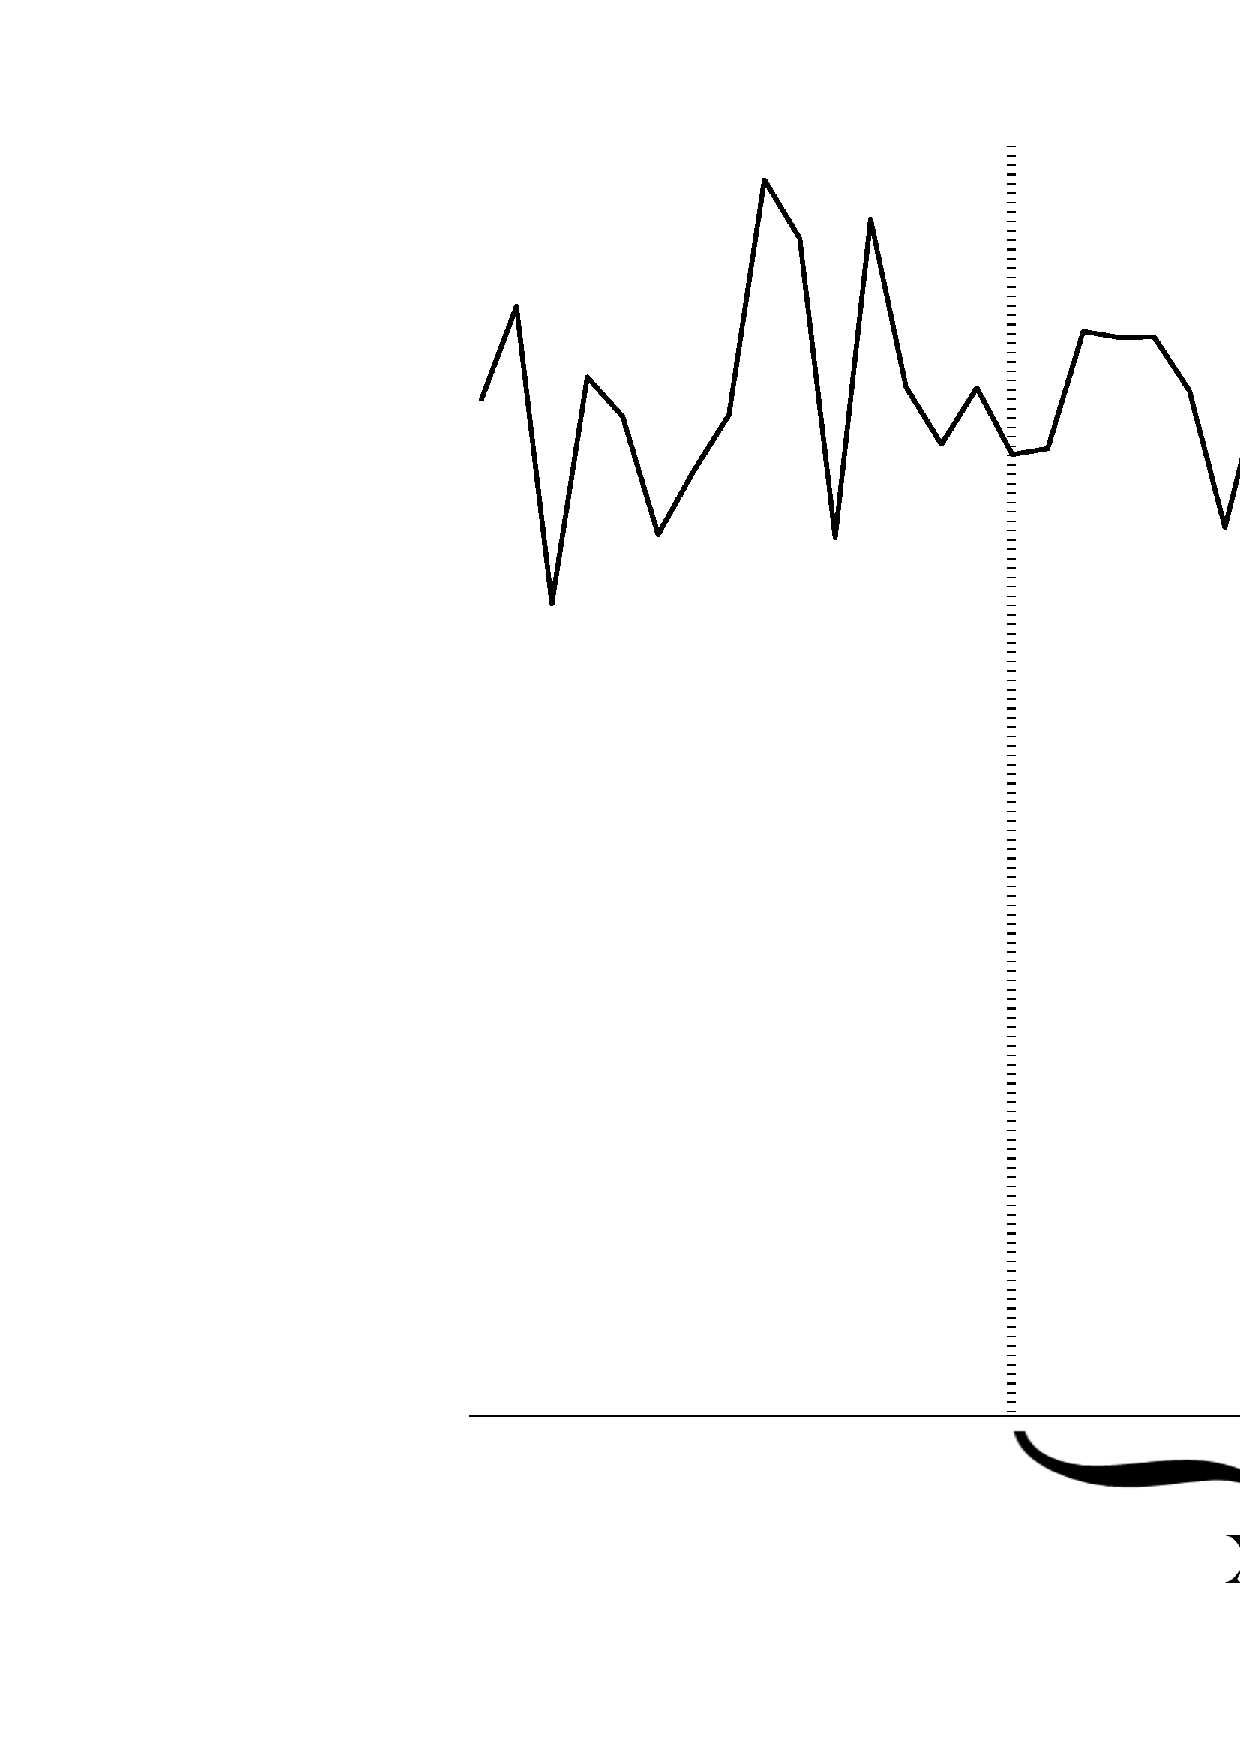
\includegraphics[scale=0.8]{cpd_ref_test.png}
 \caption{Change Point Detection}
 \label{fig:cpd_ref_test.png}
\end{figure}

Model-based approaches to change point detection assume that each tick in
a time series is a draw from some underlying probability distribution.
Scores are generated by estimating the distribution of the reference data
and the test data, and then by calculating the likelihood
that the two distributions are different.
Where it is reasonable to assume that the data belongs to a particular
family of distributions then parametric estimation methods have been employed
\cite{thatte11}. If no such modeling assumptions are reasonable then 
non-parametric methods have also been found to be viable \cite{matteson12}.
Finally, distance-based approaches such as Singular Spectrum Analysis
generate scores through other metrics of 
dissimilarity or difference between the reference data and the test data
\cite{moskvina03}.
Notationally, we say that for each tick $i$ in a time series:

\[
s_i = D(x_{r,i}, x_{t,i})
\]

Where $s_i$ is the score of the $i$th tick, $x_{r,i}$ is the reference
data associated with the $i$th tick, $x_{t,i}$ is the test data
associated with the $i$th tick, and $D(A,B)$ is a function that computes the
dissimiliarity between a matrix of data $A$ and matrix of data $B$, and is
particular to the given change point algorithm. Note that for a given
algorithm it may not be possible to generate scores right at the very beginning
of the time series (insufficient reference data) or at the very end of a time
series (insufficient test data).

\section{Methodology}

There are many different modeling assumptions and associated algorithms
for generating change point detection scores, and one simple baseline approach that we 
wanted to test was the Shewhart Control Chart. This approach assumes that the reference data is drawn from a
multivariate normal distribution, and that scores are calculated by the Mahalanobis
distance of the target time tick from the estimated multivariate normal:

\[
s_i = \sqrt{(\bar{x}_{r,i} - x_i)^T \, S_{r,i}^{-1} \, (\bar{x}_{r,i} - x_i)}
\]

where $\bar{x}_{r,i}$ is the sample mean of the reference data, $S_{r,i}$
is the sample covariance matrix of the reference data, and $x_i=x_{t,i}$ is
the $i$th data point \cite{shewhart26}.

We were also interested in testing the performance of a newer and more
sophisticated change point detection algorithm: the
Kullback-Leibler Importance Estimation Procedure (KLIEP),
introduced by Kawahara and Sugiyama \cite{sugiyama09} \cite{sugiyama08}.
This approach generates scores using the Kullback-Leibler (KL)
divergence between the reference data and the test data. One method of doing this
is to estimate the density of the reference distribution and test distribution
separately, and then compare them using a likelihood ratio
(known in the change point detection literature as \emph{importance}). 
Instead, KLIEP estimates the importance directly using a non-parametric model.

Let the estimate of the importance $\hat{R}$ be represented by this model:

\[
\hat{R} = \frac{p_{t}}{\hat{p}_{r}} = \sum_{j=1}^{n_{t}} \alpha_j K_G(x,x_{t,j})
\]

Where $p_{r}$ and $p_{t}$ are the probability densities of the reference data and the test
data, $n_{t}$ is the number of ticks in the test window, $\alpha$ is a
vector of model parameters to solve for, $x$ is the concatenation of the reference and the
test data, $x_{t,j}$ is the $j$th element of the test data,
and $K_G(A,B)$ is the Gaussian kernel with width $\sigma$:

\[
K_G(A,B) = \exp \left(-\frac{||A-B||^2}{2\sigma^2}\right)
\]

Now solve for $\alpha$ so that the empirical KL divergence between $\hat{p}_{t}$ and
$p_{t} = p_{r}\hat{R}$ is minimized, which is equivalent to the following convex optimization
problem:

\[
\begin{dcases}
 \max_{\alpha} \quad \sum_{j=1}^{n_t} \, \log \left( \sum_{k=1}^{n_t} \alpha_k K_G(x_{t,j}, x_{t,k}) \right) \\
 \,\, \text{s.t.} \quad\, \frac{1}{n_r} \sum_{j=1}^{n_r} \sum_{k=1}^{n_t} \alpha_k K_G(x_{r,j},x_{t,k}) = 1 \\
 \qquad \quad \text{and} \; \alpha_1 \ldots \alpha_{n_t} \ge 1
\end{dcases}
\]

Finally, the scores that we wish to generate are just the estimate of the importance given by the
solution to the complex optimization problem, i.e. $s_i = \hat{R}_i$.

Since this approach uses a Gaussian kernel, it requires the selection of
a kernel width $\sigma$ for each time tick. We used an implementation of
KLIEP that is available at Sugiyama's website, which included a cross-validation
procedure for the value of $\sigma$. The CV procedure chooses a number of disjoint
splits of the test data along with a number of different candidate $\sigma$'s, and runs
KLIEP with each combination of split and candidate $\sigma$. Then it chooses the candidate $\sigma$
that, on the average across all of the splits, maximizes the KL divergence (the
$\max_{\alpha}$ equation above) the most.

For the OSU Hip dataset, we used this
CV to choose the the kernel width at each individual time tick. This computationally-
intensive approach was impractical for the UQ dataset because it is orders of magnitude larger,
so instead of running it on every tick of that data, we ran the CV procedure on a number of
random ticks drawn from the data. From this we were able
to empirically identify 0.01 as a plausible $\sigma$, and so fixed $\sigma$
at that value for our experiments on this dataset.
Our reference windows were fixed at a length of 10 seconds, and our test
windows were fixed at a length of 1 second.

Once scores were generated, we chose a number of threshold values to determine which
scores were considered high enough to predict a changepoint.
Threshold values were chosen by considering the false positive rates of
change prediction for the change point detection algorithms. A smaller false positive rate
corresponded to a higher and more conservative threshold, which split the
time series into fewer segments for featurization. A larger false positive rate
corresponded to a lower threshold, which split the time series into more segments.

\section{Results}
Figure \ref{fig:cpd_perf}, shows accuracy and detection time as a function of the
false positive rate per second, for the OSU Hip dataset,
for each of the SVM, Decision Tree, and Neural Net base classifiers.

\begin{figure}
 \centering
 \includegraphics[scale=0.3]{osu_cpd_dt_acc.png}
 \includegraphics[scale=0.3]{osu_cpd_svm_acc.png}
 \includegraphics[scale=0.3]{osu_cpd_nnet_acc.png}
 \includegraphics[scale=0.3]{osu_cpd_dt_det.png}
 \includegraphics[scale=0.3]{osu_cpd_svm_det.png}
 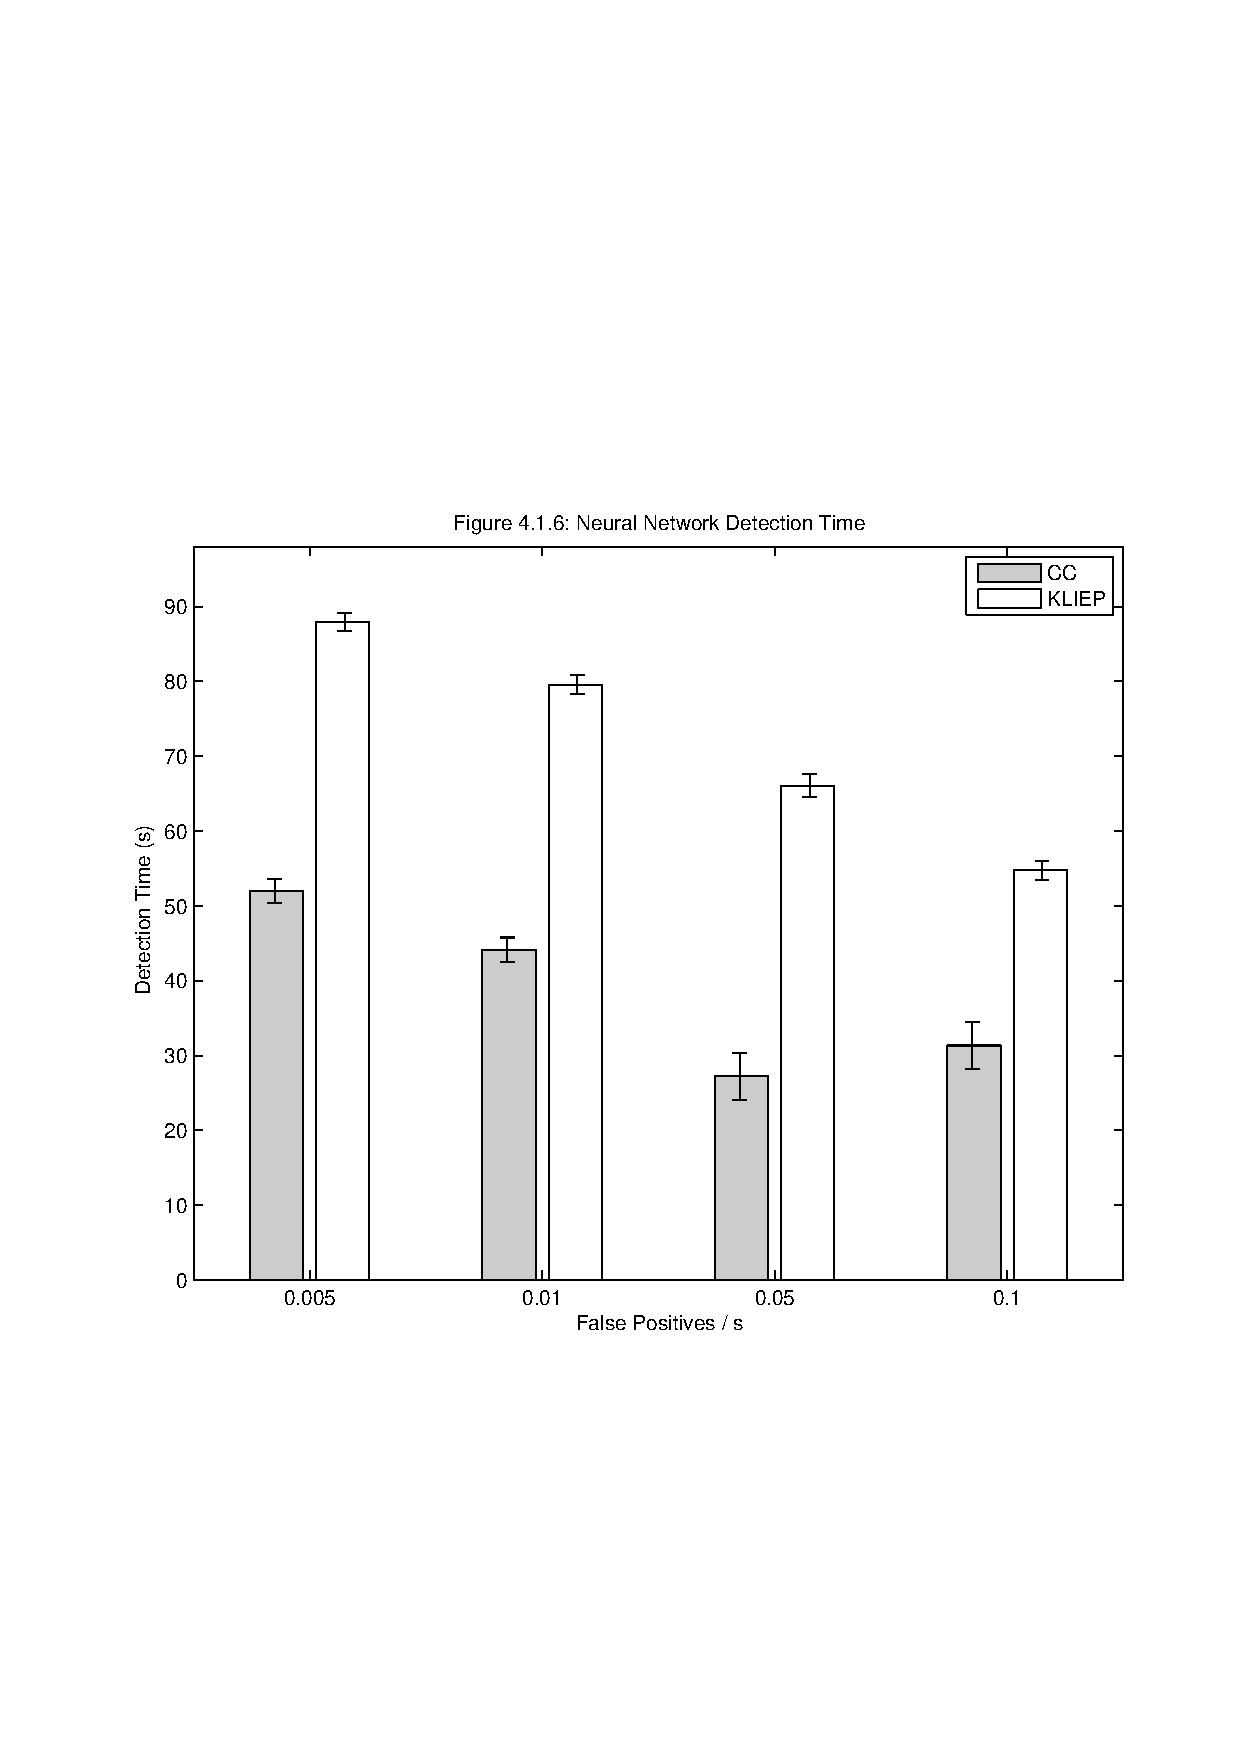
\includegraphics[scale=0.3]{osu_cpd_nnet_det.png}
 \caption{CPD-Based Classification Performance}
 \label{fig:cpd_perf}
\end{figure}

\section{Discussion}


\input(bottomup}

%\chapter{Results}
%Figure \ref{fig:cpd_perf}, shows accuracy and detection time as a function of the
%false positive rate per second, for the OSU Hip dataset,
%for each of the SVM, Decision Tree, and Neural Net base classifiers.
%
%\begin{figure}
% \centering
% \includegraphics[scale=0.3]{osu_cpd_dt_acc.png}
% \includegraphics[scale=0.3]{osu_cpd_svm_acc.png}
% \includegraphics[scale=0.3]{osu_cpd_nnet_acc.png}
% \includegraphics[scale=0.3]{osu_cpd_dt_det.png}
% \includegraphics[scale=0.3]{osu_cpd_svm_det.png}
% 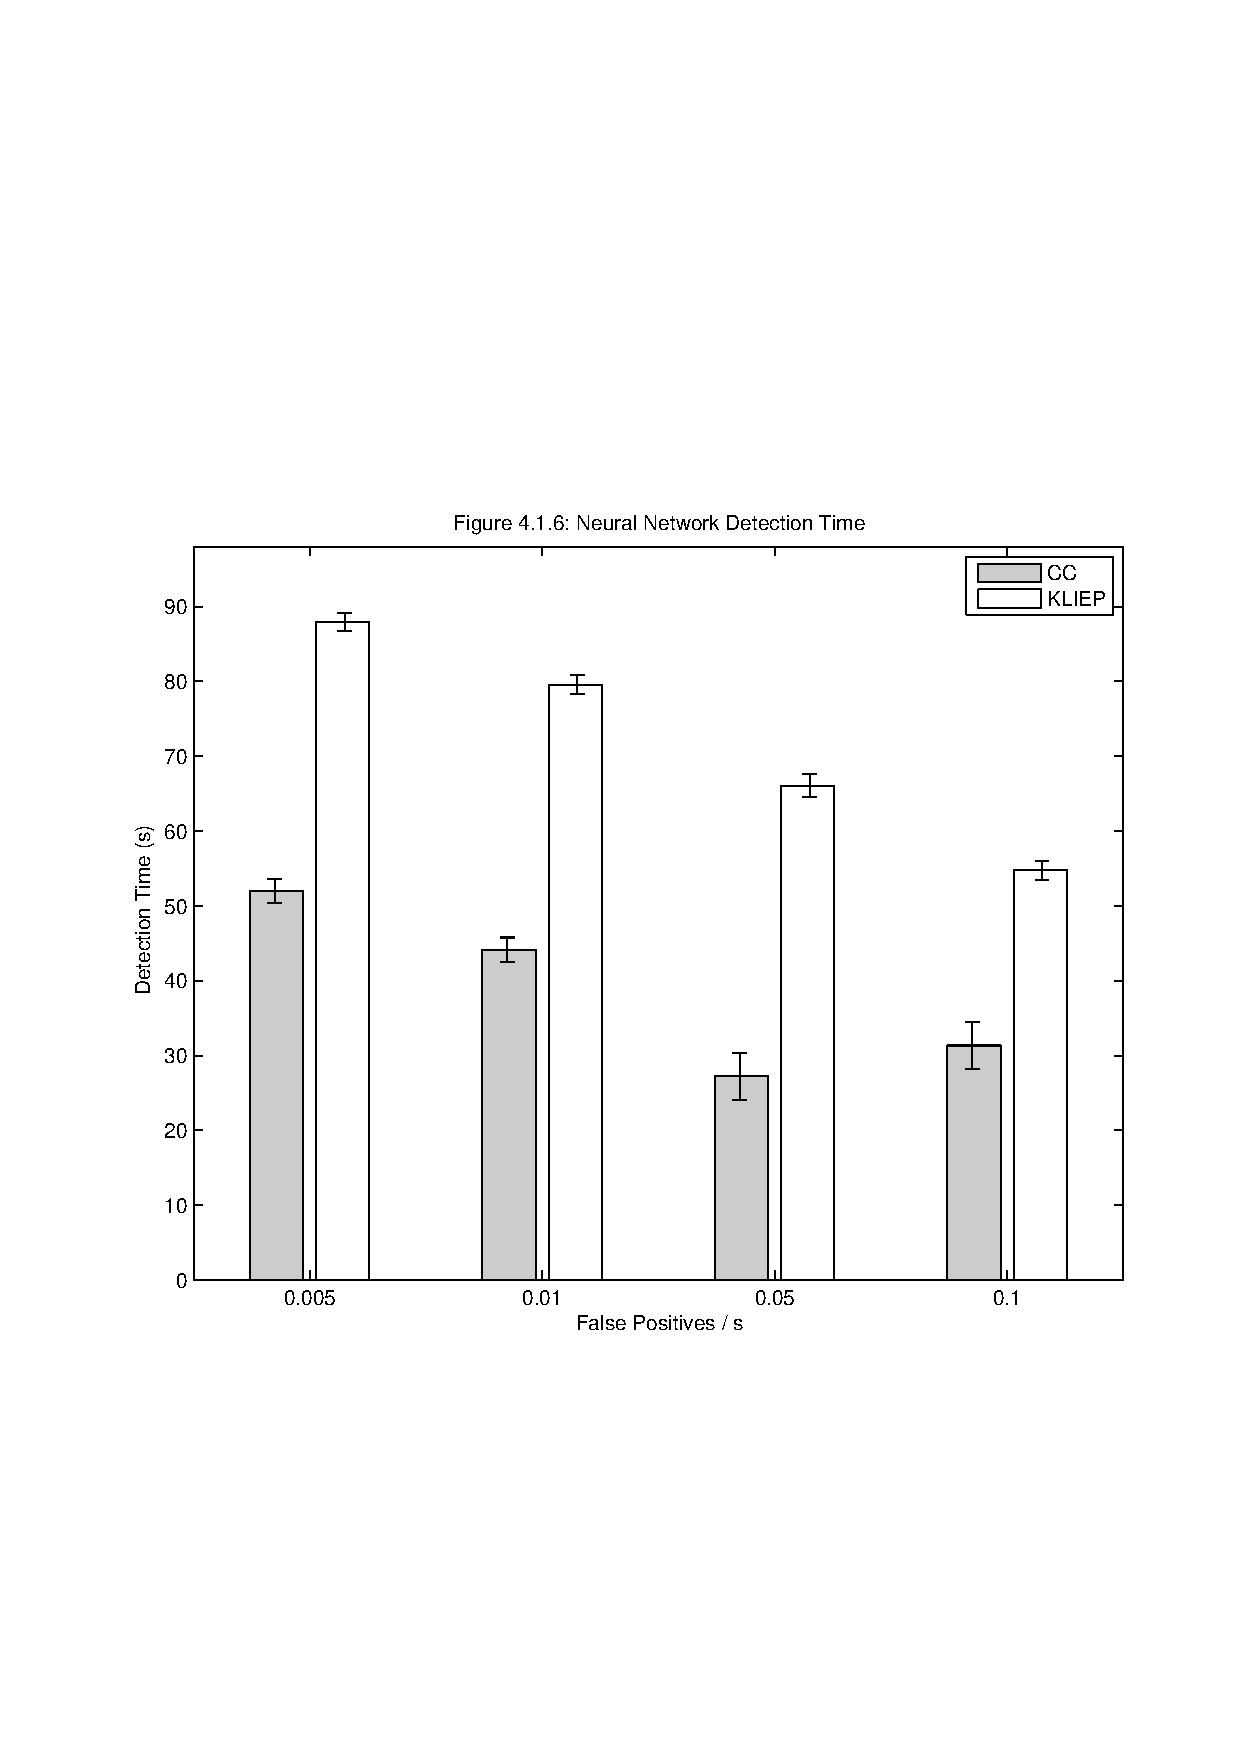
\includegraphics[scale=0.3]{osu_cpd_nnet_det.png}
% \caption{CPD-Based Classification Performance}
% \label{fig:cpd_perf}
%\end{figure}

\section{Change-Point Detection}
Results for our change-point detection experiments are given in
Figures \ref{fig:osu_cpd}-\ref{fig:lime2_cpd}.
We hypothesized that the performance of the change-point detection algorithms
would depend heavily on the threshold level for change prediction. This was
tested by varying the average number of times per second that the algorithms
falsely predicted a change. A large number of such false positive rates per
second were tested, but for the sake of brevity only a representative sample
of $\{0.005, 0.01, 0.05, 0.1\}$ are shown here.

In the OSU Hip experiments, control charts outperformed KLIEP in terms of
detection time (Figures 4.1.2, 4.1.4, 4.1.6), while the accuracy results were
mixed. It is generally expected that the accuracy curve as
a function of the false positive rate will be unimodal: very large windows
extend into multiple activities and confuse a classifier, while very small
windows do not contain enough information to be discriminative. This
unimodal behavior is shown in the control chart results, but not in the KLIEP
results (Figures 4.1.1, 4.1.3, 4.1.5). Follow-up experiments showed that the peak
in KLIEP accuracy performance occurred between false positive rates of $0.2$ and
$0.3$ for each of the three classifiers.

Further investigation indicated that across the OSU Hip dataset the KLIEP algorithm
was unable to detect many different activity changes without a very low score
threshold value (and consequently very high false positive rates).
Some qualitative plotting of the OSU Hip data showed
that most of its activities have accelerometer amplitude values that strongly
resemble draws from a multivariate normal distribution. Since control charts
assume that the data is drawn from a distribution that is a member of that
family, it is logical that control charts would outperform algorithms with
different modeling assumptions on OSU Hip.

In the LiME experiments, KLIEP outperformed control charts in terms of
accuracy across the board, and control charts outperformed KLIEP in terms of
detection time across the board. (TODO: Need to interpret this, but not sure
how.)

Finally, in a few cases (Figures 4.1.2, 4.1.6, 4.2.6) the detection time did
not decrease as the false positive rate increased. On the face of it this would seem
to be a non-sequitur, but this only happened in cases when accuracy also decreased
(Figures 4.1.1, 4.1.5, 4.2.5).
Smaller window sizes tend to be correlated with decreased detection times, but
it is possible that predicting on smaller windows, if they happen to be less discriminative,
can actually increase the time required for the classifier to start correctly
predicting the ground-truth activity. Additionally, the given increases in detection
time were small and near standard error.

%\setlength{\abovecaptionskip}{-5pt}

\begin{table}[h]
\captionsetup{font=scriptsize}
\begin{center}
\tiny{
\begin{tabular}{ cc|c|c|c|c|c|c|c|c|c|c|c|c| }
\cline{3-14}
& & \multicolumn{4}{ c| }{DT} & \multicolumn{4}{ c| }{SVM} & \multicolumn{4}{ c| }{NNET}\\ \cline{3-14}
& & 0.005 & 0.01 & 0.05 & 0.1 & 0.005 & 0.01 & 0.05 & 0.1 & 0.005 & 0.01 & 0.05 & 0.1\\ \cline{1-14}
\multicolumn{1}{ |c| }{\multirow{2}{*}{OSU Hip}} &
\multicolumn{1}{ |c| }{CC} & 49.2 & 46.8 & 38.9 & 35.4 & 66.8 & \textbf{67.9} & 55.2 & 47.0 & 62.3 & 65.9 & 64.5 & 53.1\\ \cline{2-14}
\multicolumn{1}{ |c }{} &
\multicolumn{1}{ |c| }{KLIEP} & 31.0 & 32.3 & 36.9 & 41.3 & 40.3 & 44.3 & 52.1 & 58.0 & 41.0 & 43.8 & 53.0 & \textbf{59.9}\\ \cline{1-14}
\multicolumn{1}{ |c| }{\multirow{2}{*}{LiME Day 1}} &
\multicolumn{1}{ |c| }{CC} & 47.5 & 48.2 & 43.0 & 41.9 & \textbf{57.7} & 57.3 & 52.0 & 51.4 & 19.1 & 21.0 & 17.4 & 16.8\\ \cline{2-14}
\multicolumn{1}{ |c }{} &
\multicolumn{1}{ |c| }{KLIEP} & 58.8 & 57.6 & 53.8 & 52.3 & \textbf{68.7} & 66.7 & 61.9 & 59.2 & 23.6 & 20.8 & 22.9 & 19.0\\ \cline{1-14}
\multicolumn{1}{ |c| }{\multirow{2}{*}{LiME Day 2}} &
\multicolumn{1}{ |c| }{CC} & \textbf{54.0} & 53.6 & 50.3 & 50.2 & 53.3 & 52.5 & 49.5 & 45.9 & 21.6 & 19.7 & 17.3 & 15.4\\ \cline{2-14}
\multicolumn{1}{ |c }{} &
\multicolumn{1}{ |c| }{KLIEP} & 63.4 & 61.5 & 59.0 & 58.6 & \textbf{65.5} & 63.2 & 58.1 & 55.8 & 25.6 & 20.0 & 20.1 & 19.6\\ \cline{1-14}
\end{tabular}
}
\end{center}
\caption{CPD Accuracy}
\label{tbl:cpd_acc}
\end{table}

\begin{table}[h]
\captionsetup{font=scriptsize}
\begin{center}
\tiny{
\begin{tabular}{ c|c|c|c|c|c|c| }
\cline{2-7}
 & \multicolumn{2}{ c| }{DT} & \multicolumn{2}{ c| }{SVM} & \multicolumn{2}{ c| }{NNET}\\ \cline{2-7}
 & 20 & 10 & 20 & 10 & 20 & 10\\ \cline{1-7}
\multicolumn{1}{ |c| }{OSU Hip}
 & 89.5 & 88.1 & \textbf{94.9} & 94.4 & 71.2 & 62.2\\ \cline{1-7}
\multicolumn{1}{ |c| }{LiME Day 1}
 & 84.3 & 83.3 & 78.3 & \textbf{84.8} & 69.6 & 51.7\\ \cline{1-7}
\multicolumn{1}{ |c| }{LiME Day 2}
 & \textbf{87.5} & 85.6 & 79.4 & 86.4 & 57.7 & 78.4\\ \cline{1-7}
\end{tabular}
}
\end{center}
\caption{HMM Accuracy}
\label{tbl:hmm_acc}
\end{table}

\begin{table}[h]
\captionsetup{font=scriptsize}
\begin{center}
\tiny{
\begin{tabular}{ cc|c|c|c|c|c|c|c|c|c|c|c|c| }
\cline{3-14}
& & \multicolumn{4}{ c| }{DT} & \multicolumn{4}{ c| }{SVM} & \multicolumn{4}{ c| }{NNET}\\ \cline{3-14}
& & 0.005 & 0.01 & 0.05 & 0.1 & 0.005 & 0.01 & 0.05 & 0.1 & 0.005 & 0.01 & 0.05 & 0.1\\ \cline{1-14}
\multicolumn{1}{ |c| }{\multirow{2}{*}{OSU Hip}} &
\multicolumn{1}{ |c| }{CC} & 69.7 & 66.5 & 68.8 & 70.7 & 49.3 & 42.2 & 35.9 & 35.0 & 52.0 & 44.2 & \textbf{27.2} & 31.3\\ \cline{2-14}
\multicolumn{1}{ |c }{} &
\multicolumn{1}{ |c| }{KLIEP} & 101.6 & 98.9 & 94.0 & 88.5 & 87.1 & 81.6 & 71.8 & 63.3 & 86.9 & 78.6 & 65.1 & \textbf{53.8}\\ \cline{1-14}
\multicolumn{1}{ |c| }{\multirow{2}{*}{LiME Day 1}} &
\multicolumn{1}{ |c| }{CC} & 107.2 & 76.9 & 56.0 & 51.3 & 79.1 & 55.5 & 36.6 & \textbf{32.8} & 168.8 & 111.1 & 78.2 & 76.8\\ \cline{2-14}
\multicolumn{1}{ |c }{} &
\multicolumn{1}{ |c| }{KLIEP} & 146.1 & 116.0 & 59.7 & 50.9 & 113.5 & 88.7 & 43.8 & \textbf{36.0} & 237.9 & 191.4 & 92.5 & 82.3\\ \cline{1-14}
\multicolumn{1}{ |c| }{\multirow{2}{*}{LiME Day 2}} &
\multicolumn{1}{ |c| }{CC} & 103.7 & 80.4 & 59.8 & 54.3 & 101.8 & 72.2 & 52.1 & \textbf{48.8} & 161.5 & 130.2 & 78.6 & 72.0\\ \cline{2-14}
\multicolumn{1}{ |c }{} &
\multicolumn{1}{ |c| }{KLIEP} & 136.0 & 121.3 & 63.2 & 54.8 & 127.3 & 112.3 & 58.4 & \textbf{50.4} & 242.6 & 216.6 & 109.2 & 88.3\\ \cline{1-14}
\end{tabular}
}
\end{center}
\caption{CPD Detection Time}
\label{tbl:cpd_det}
\end{table}

\begin{table}[h]
\captionsetup{font=scriptsize}
\begin{center}
\tiny{
\begin{tabular}{ c|c|c|c|c|c|c| }
\cline{2-7}
 & \multicolumn{2}{ c| }{DT} & \multicolumn{2}{ c| }{SVM} & \multicolumn{2}{ c| }{NNET}\\ \cline{2-7}
 & 20 & 10 & 20 & 10 & 20 & 10\\ \cline{1-7}
\multicolumn{1}{ |c| }{OSU Hip}
 & 9.8 & 9.8 & 4.5 & \textbf{4.2} & 31.4 & 40.1\\ \cline{1-7}
\multicolumn{1}{ |c| }{LiME Day 1}
 & 57.1 & 32.2 & 103.5 & \textbf{25.0} & 177.7 & 146.3\\ \cline{1-7}
\multicolumn{1}{ |c| }{LiME Day 2}
 & 47.8 & \textbf{31.7} & 101.2 & 31.8 & 255.5 & 53.7\\ \cline{1-7}
\end{tabular}
}
\end{center}
\caption{HMM Detection Time}
\label{tbl:hmm_det}
\end{table}

\setlength{\abovecaptionskip}{10pt}


\begin{figure}[H]
 \includegraphics[scale=0.4]{osu_cpd_dt_acc.pdf} \hspace{1em}\vspace{1em}
 \includegraphics[scale=0.4]{osu_cpd_dt_det.pdf}
 \includegraphics[scale=0.4]{osu_cpd_svm_acc.pdf} \hspace{1em}\vspace{1em}
 \includegraphics[scale=0.4]{osu_cpd_svm_det.pdf}
 \includegraphics[scale=0.4]{osu_cpd_nnet_acc.pdf} \hspace{2em}
 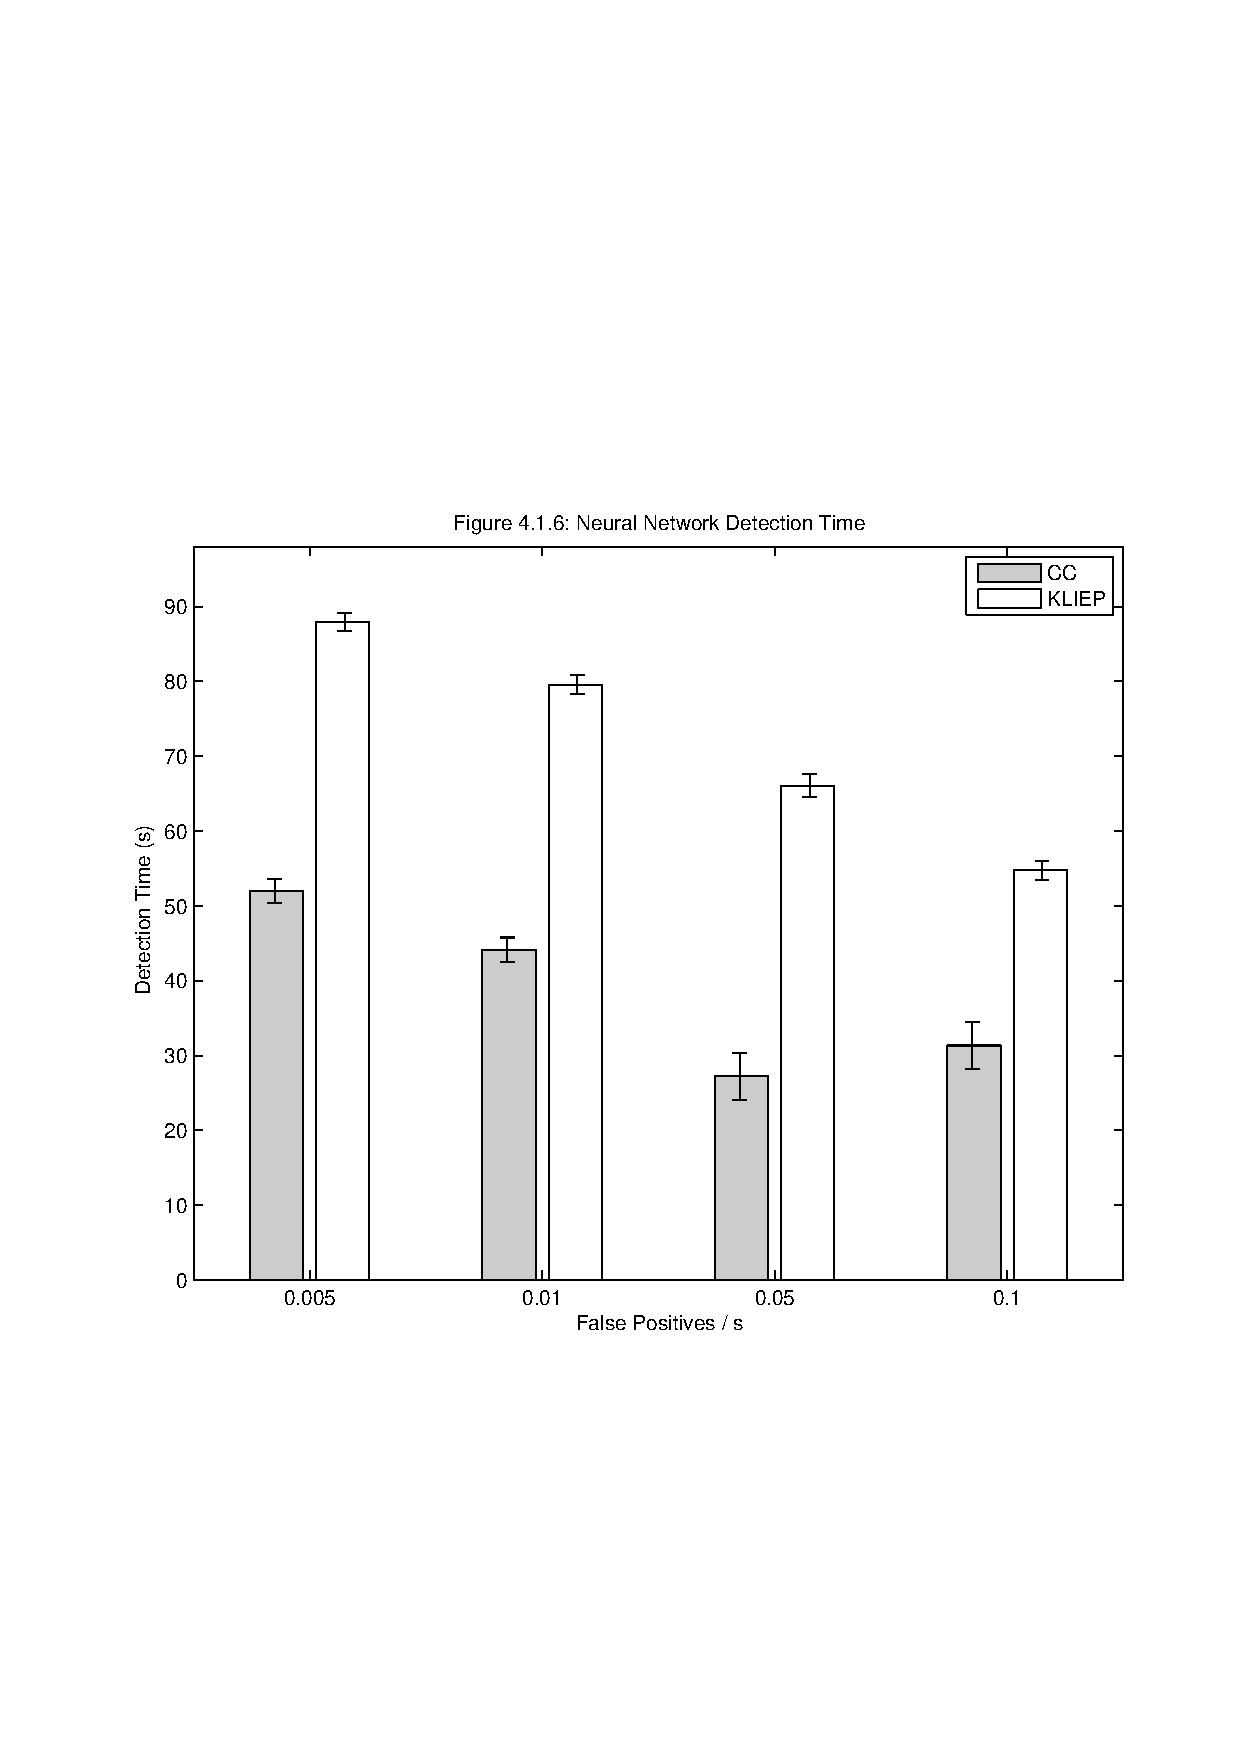
\includegraphics[scale=0.4]{osu_cpd_nnet_det.pdf}
 \caption{OSU Hip Results. Graphs are organized into rows by base classifier,
  and columns by evaluation metric. Change-point detection result were averaged over
  30 splits into training, testing, and validation datasets,
  along with bars showing one standard error.}
 \label{fig:osu_cpd}
\end{figure}

\begin{figure}[H]
 \centering
 \includegraphics[scale=0.4]{lime1_cpd_dt_acc.pdf} \hspace{1em}\vspace{1em}
 \includegraphics[scale=0.4]{lime1_cpd_dt_det.pdf}
 \includegraphics[scale=0.4]{lime1_cpd_svm_acc.pdf} \hspace{1em}\vspace{1em}
 \includegraphics[scale=0.4]{lime1_cpd_svm_det.pdf}
 \includegraphics[scale=0.4]{lime1_cpd_nnet_acc.pdf} \hspace{1em}
 \includegraphics[scale=0.4]{lime1_cpd_nnet_det.pdf}
 \caption{LiME Day 1 Results}
 \label{fig:lime1_cpd}
\end{figure}

\begin{figure}[H]
 \centering
 \includegraphics[scale=0.4]{lime2_cpd_dt_acc.pdf} \hspace{1em}\vspace{1em}
 \includegraphics[scale=0.4]{lime2_cpd_dt_det.pdf}
 \includegraphics[scale=0.4]{lime2_cpd_svm_acc.pdf} \hspace{1em}\vspace{1em}
 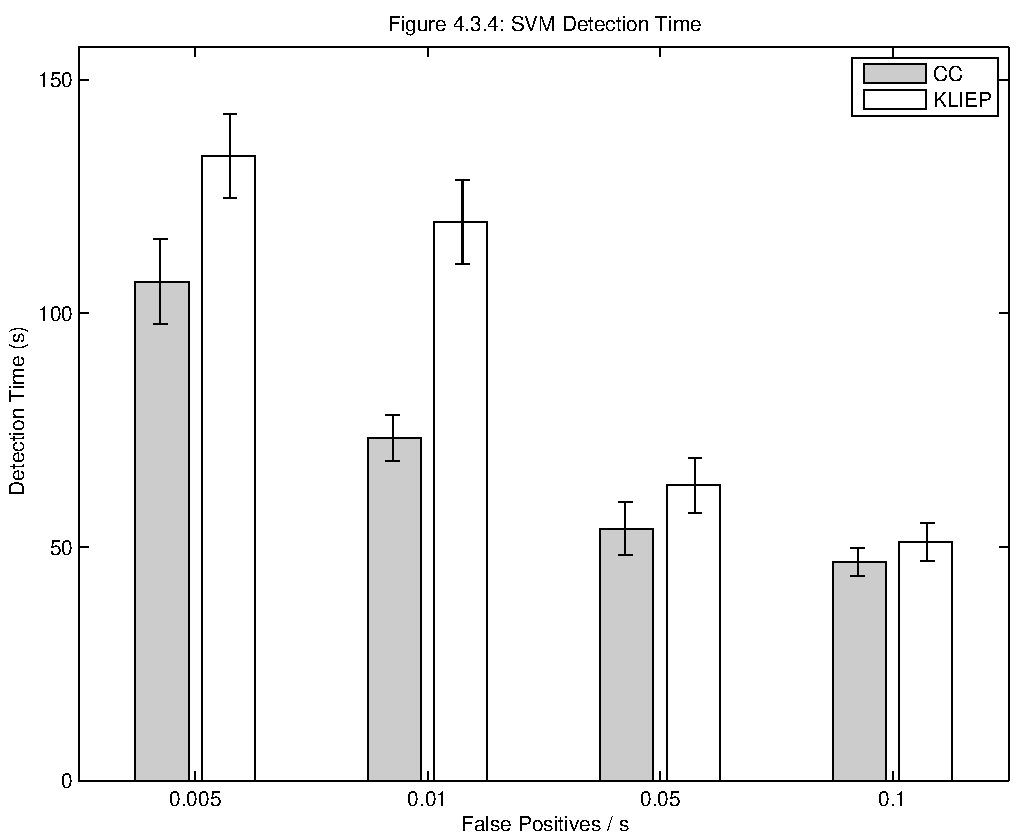
\includegraphics[scale=0.4]{lime2_cpd_svm_det.pdf}
 \includegraphics[scale=0.4]{lime2_cpd_nnet_acc.pdf} \hspace{1em}
 \includegraphics[scale=0.4]{lime2_cpd_nnet_det.pdf}
 \caption{LiME Day 2 Results}
 \label{fig:lime2_cpd}
\end{figure}


\section{HMM}

Results for our HMM experiments are given in
Figures \ref{fig:osu_hmm}-\ref{fig:lime2_hmm}. Each HMM experiment was
performed by splitting time series into windows of fixed length for
featurization, and results for windows of length $\{10, 12, 14, 16, 18, 20\}$
seconds are shown.

For both the SVM and decision tree classifiers, accuracy and detection time
was strong across all three datasets, and also stable with respect to window
size. Further experiments on the OSU Hip dataset showed that the HMM when
paired with these classifiers
tends to be stable with window sizes that are greater than a few seconds,
which seems to be the amount of time required to be informative. Neural networks
performed somewhat more poorly and erratically across the board.

\begin{figure}[H]
 \centering
 \includegraphics[scale=0.4]{osu_hmm_dt_acc.pdf} \hspace{1em}\vspace{1em}
 \includegraphics[scale=0.4]{osu_hmm_dt_det.pdf}
 \includegraphics[scale=0.4]{osu_hmm_svm_acc.pdf} \hspace{1em}\vspace{1em}
 \includegraphics[scale=0.4]{osu_hmm_svm_det.pdf}
 \includegraphics[scale=0.4]{osu_hmm_nnet_acc.pdf} \hspace{1em}
 \includegraphics[scale=0.4]{osu_hmm_nnet_det.pdf}
 \caption{OSU Hip HMM Results.
  Graphs are organized into rows by base classifier, and columns by evaluation
  metric. HMM results were averaged over 10 splits into training
  (base classifier), validation, training (HMM), and testing datasets, along with bars
  showing one standard error.}
 \label{fig:osu_hmm}
\end{figure}

\begin{figure}[H]
 \centering
 \includegraphics[scale=0.4]{lime1_hmm_dt_acc.pdf} \hspace{1em}\vspace{1em}
 \includegraphics[scale=0.4]{lime1_hmm_dt_det.pdf} 
 \includegraphics[scale=0.4]{lime1_hmm_svm_acc.pdf} \hspace{1em}\vspace{1em}
 \includegraphics[scale=0.4]{lime1_hmm_svm_det.pdf} 
 \includegraphics[scale=0.4]{lime1_hmm_nnet_acc.pdf} \hspace{1em}
 \includegraphics[scale=0.4]{lime1_hmm_nnet_det.pdf} 
 \caption{LiME Day 1 HMM Results}
 \label{fig:lime1_hmm}
\end{figure}

\begin{figure}[H]
 \centering
 \includegraphics[scale=0.4]{lime2_hmm_dt_acc.pdf} \hspace{1em}\vspace{1em}
 \includegraphics[scale=0.4]{lime2_hmm_dt_det.pdf}
 \includegraphics[scale=0.4]{lime2_hmm_svm_acc.pdf} \hspace{1em}\vspace{1em}
 \includegraphics[scale=0.4]{lime2_hmm_svm_det.pdf}
 \includegraphics[scale=0.4]{lime2_hmm_nnet_acc.pdf} \hspace{1em}
 \includegraphics[scale=0.4]{lime2_hmm_nnet_det.pdf}
 \caption{LiME Day 2 HMM Results}
 \label{fig:lime2_hmm}
\end{figure}

\newpage

\section{Discussion}

Our results clearly show that the HMM approach outperformed the change-point
detection approach, both in terms of accuracy and detection time, regardless of
the dataset and base classifier. This was expected, as our change-point
detection algorithms did not perform expecially well at predicting changes at
the correct locations, and also because HMMs are a well-established and well-
grounded approach in sequential, time-oriented domains.

A further point of interest was that SVM clearly beat out the other two
base classifiers, and that the faster and simpler decision tree model did fairly
well against neural networks. This result is significant because much of the
previous research that has formulated activity detection as a supervised learning
problem has used neural networks exclusively.

